% Requires: booktabs, tabularx, graphicx, amsmath, tikz; \newcommand{\pc}{p_C}
\providecommand{\pc}{p_C}

\section{Method: what we do and how it works}
\label{sec:method}

\subsection{The problem}
In a social network, accounts cluster into follow-graph communities. Most accounts say things that fit the community they sit in. Some do not: their bio and posts read like those of another community. We call these accounts \emph{misfits}. A misfit may be a bridge between communities, a recruiter, an infiltrator, or simply a user the follow graph under-serves. Finding such accounts matters for two reasons. First, they are candidates for bad actors that centrality scores do not single out. Second, they are natural targets for \emph{re-homing}: steering their ties toward the community their text points to, for example by recommending links or rewiring follows, so that corrections and other content reach them. The method needs no labels. It uses only the graph and each account's text.

\begin{figure}[htbp]
\centering
\begin{tikzpicture}[
  box/.style={draw, rounded corners, align=center, minimum height=1.0cm,
              text width=2.4cm, font=\footnotesize},
  arr/.style={-{Latex[length=2mm]}, thick},
  node distance=0.5cm and 0.55cm]
  \node[box] (graph) at (0,0) {Follow graph};
  \node[box] (text) at (0,-2.1) {Account text\\(bio)};
  \node[box] (leiden) at (3.25,0) {Leiden\\communities $t$};
  \node[box] (clf) at (3.25,-2.1) {MiniLM $\to$ cross-fitted classifier $p_C$};
  \node[box] (misfit) at (6.5,-1.05) {Misfit score\\$1-p_C[i,t_i]$};
  \node[box] (target) at (9.75,-1.05) {Target $\tau_i$\\$\arg\max_c p_C[i,c]$};
  \node[box] (eng) at (13.0,0) {Engagement\\check};
  \node[box] (rew) at (13.0,-2.1) {Rewiring\\and cascade};

  \draw[arr] (graph) -- (leiden);
  \draw[arr] (text) -- (clf);
  \draw[arr] (leiden) -- node[left, font=\scriptsize] {labels $t$} (clf);
  \draw[arr] (leiden) -- (misfit);
  \draw[arr] (clf) -- (misfit);
  \draw[arr] (misfit) -- (target);
  \draw[arr] (target) -- (eng);
  \draw[arr] (target) -- (rew);
\end{tikzpicture}
\caption{Pipeline. Communities come from the graph alone. The classifier sees only text; the community labels $t$ are its training targets, and cross-fitting means no node's own label informs its own prediction. The misfit score compares the two views, and the target $\tau_i$ is where the text says the node belongs.}
\label{fig:pipeline}
\end{figure}

\subsection{How it works}
\paragraph{Communities.}
Let $G$ be the social graph and $t_i$ the community of node $i$ found by Leiden \cite{traag2019leiden} (best of 100 runs).

\paragraph{Text classifier.}
Let $x_i$ be the node's text embedding (sentence embeddings \cite{reimers2019sbert}, 384-d MiniLM). A text-only logistic-regression classifier is trained to predict $t$ from $x$. To keep a node's own label from informing its own score, the classifier is \emph{cross-fitted}: each node is scored by a model trained on the other folds (5-fold). This yields $\pc[i,c]$, the probability that node $i$'s text belongs to community $c$.

\paragraph{Misfit and disagreement scores.}
The misfit score is one minus the probability that the text places the node in its own community,
\begin{equation}
\mathrm{misfit}_i = 1 - \pc[i,\,t_i].
\label{eq:misfit}
\end{equation}
A second score, \emph{disagreement}, is the Jensen--Shannon divergence between $\pc[i,\cdot]$ and a structural membership $p_T[i,\cdot]$ obtained from label spread over the Leiden runs. It follows the ambiguity idea of Sani et al.~\cite{sani2025aas}, applied to nodes rather than images. A high score marks a node whose graph position and text disagree.

\paragraph{Leak control.}
Real text can contain the community signal directly (for example, a latest tweet about a party). Where the dataset allows, we therefore evaluate with bio-only text as the valid setting, and treat richer text (bio plus latest tweet, GloVe) only as a leak-control reference.

\paragraph{Re-homing target.}
For node $i$ the target community is the one its text fits best,
\begin{equation}
\tau_i = \arg\max_c \pc[i,c].
\label{eq:target}
\end{equation}
Re-homing means steering the node's ties toward $\tau_i$, either as link recommendations or as rewiring.

\paragraph{Rewiring and cascade reach.}
For each treated (misfit) node, \meth{rehome\_text} drops up to $k$ dormant own-community follow edges and adds the same number of edges into $\tau_i$, which keeps degrees unchanged. We then simulate cascades with weighted-cascade acceptance (\meth{wc}, $p{=}1/\text{in-degree}$) \cite{kempe2003influence} and a content-gating strength $\beta$: a node accepts content from its own community more readily by a factor $e^{\beta}$. \emph{Correction reach} is the share of nodes reached by correcting content, in percentage points (pp).

\paragraph{Data.}
\emph{TIMME} \cite{xiao2020timme}: 20{,}811 Twitter accounts with bios, tweets, and follow, retweet, like and mention layers. \emph{Pokec slice}: a regional slice of the SNAP Pokec network \cite{snap} with interest text and profile fields. \emph{Synthetic}: a degree-corrected stochastic block model ($n{=}4000$, $K{=}8$) with planted mismatched nodes; $\mu$ is community mixing, $\sigma$ text noise, and ``nuisance'' the strength of a community-blind text block. The real graphs have genuine community structure: Louvain modularity $Q$ is 0.256 (TIMME) and 0.49 (Pokec slice), against 0.035 and 0.206 for a degree-preserving rewired null. On TIMME, text predicts the Leiden community well above the majority rate (0.622 vs 0.318).

\section{Where it performs well}
\label{sec:perform}
Three results are supported by the evidence: misfit finds planted mismatches far better than every comparator, the text-predicted community is where misfits' engagement goes, and rewiring toward it increases correction reach in simulation.

\subsection{How we judge performance}
\label{sec:judge}
Each result has its own ground truth, metric and comparators (Table~\ref{tab:comp}). We chose, for each task, the strongest relevant method available as the comparator.

\paragraph{Detection.}
The ground truth is the set of nodes whose text was planted to mismatch their community in a synthetic graph. The metric is AUC (probability that a random planted node outranks a random other node; 0.5 is chance). \emph{Degree} stands for centrality, the usual proxy for a suspicious account. \emph{Participation} and \emph{consensus entropy} are the structural-ambiguity scores: they find nodes between communities with no text at all. The \emph{content outlier} score (text far from its own community's centroid) is the text-only score: it shows whether the graph is needed. \emph{Radar} (Li et al., IJCAI 2017) \cite{li2017radar} is the standard residual-analysis anomaly detector for attributed networks and the only comparator that uses the same inputs as ours, the graph and the text attributes. We gave Radar every advantage: its parameters $(\alpha,\beta,\gamma)$ were tuned using the planted labels of one setting and reused in all.

\paragraph{Engagement.}
The ground truth is held-out cross-community retweets, likes and mentions of the top-10\% misfits. No engagement tie is used to build any predictor. The metric is the share of those ties that land in the predicted community. We compare against chance (size-weighted); the Kumari-style structural target, the non-own community where the node has most of its follow edges \cite{kumari2021deception}; one-step label propagation \cite{zhu2002label}, the standard way to infer a node's community from its neighbours; the structural membership $p_T$ (argmax over non-own communities); and Adamic--Adar \cite{adamic2003friends} summed per community. These cover the graph-only ways to guess where a node's ties should go.

\paragraph{Rewiring.}
The ground truth is a cascade simulation; the metric is correction reach in pp, with paired contrasts. Comparators: no rewiring (\meth{none}); \meth{random\_rewire} (same drops, random adds), which separates the effect of targeting from that of any rewiring; \meth{rehome\_struct}, structural re-homing in the style of Kumari et al.; and \meth{rehome\_text} applied to random nodes, which isolates the value of choosing misfits.

\paragraph{Uncertainty.}
Intervals are 95\% and always of a stated kind: paired bootstrap over simulations, bootstrap over users, or $t$-intervals over seeds. Where no spread was stored (detection: mean of 3 seeds), we show none and bold nothing.

\begin{table}[htbp]
\caption{Comparators by task.}
\label{tab:comp}
\centering\small
\begin{tabular}{@{}>{\raggedright\arraybackslash}p{0.13\linewidth}>{\raggedright\arraybackslash}p{0.15\linewidth}>{\raggedright\arraybackslash}p{0.42\linewidth}>{\raggedright\arraybackslash}p{0.22\linewidth}@{}}
\toprule
Task & Ours & Comparators & Metric\\
\midrule
Detection & misfit, disagreement & Radar, content outlier, degree, participation, consensus entropy & AUC vs planted mismatches\\
Engagement & $\arg\max\pc$ & chance, most-linked community (Kumari-style), label propagation, $p_T$, Adamic--Adar & share of held-out cross-community ties in target\\
Rewiring & \meth{rehome\_text} & \meth{none}, \meth{random\_rewire}, \meth{rehome\_struct}, \meth{rehome\_text} on random nodes & correction reach (pp), paired contrast\\
\bottomrule
\end{tabular}
\end{table}

\subsection{Detecting planted misfits}
Misfit leads every comparator in all 18 planted settings (three mixing levels, three noise levels, two nuisance levels), with AUC from 0.730 to 0.999. Fig.~\ref{fig:e05} and Table~\ref{tab:e05} show $\mu{=}0.5$. Radar stays at chance (AUC 0.49 to 0.54 over all 18 settings) even with parameters tuned on the planted labels of one setting; with its default parameters the residual collapses to about zero because the attributes are fully reconstructable (AUC 0.494 at nuisance 1.5, $\mu{=}0.5$, $\sigma{=}2$). Degree, participation and consensus entropy sit at 0.50--0.51 throughout. The advantage over the text-only score grows as the text carries community-blind variation, as real text does: at nuisance 1.5, misfit reaches 0.904 at $\sigma{=}1$ against 0.607 for content outlier. Misfit and disagreement are within 0.025 of each other and we do not rank them. This is synthetic data with three seeds and no stored spread, and the planted text mismatch is what misfit measures.

\begin{figure}[htbp]
\centering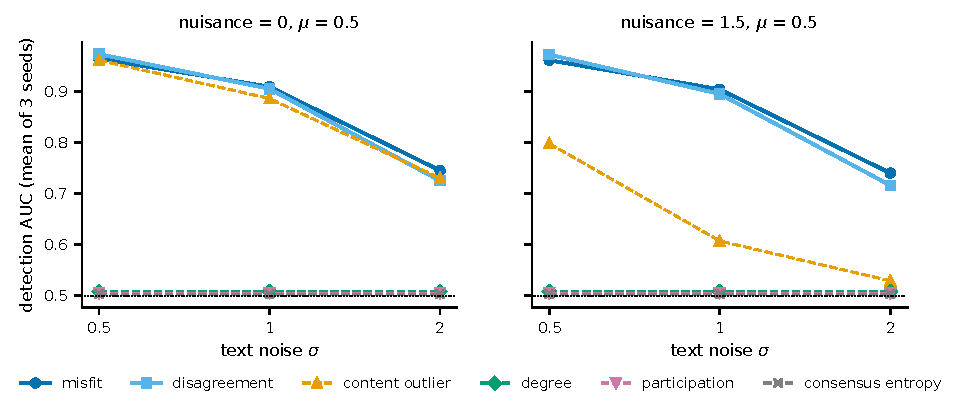
\includegraphics[width=\linewidth]{fig_e05.pdf}
\caption{Detection AUC for planted mismatches versus text noise $\sigma$ ($\mu{=}0.5$). Left: no nuisance text variation. Right: nuisance 1.5. Misfit and disagreement are ours; Radar uses parameters tuned on the planted labels. Means over 3 seeds; no spread stored.}
\label{fig:e05}
\end{figure}

\begin{table}[htbp]
\caption{Detection AUC, planted DC-SBM, $\mu{=}0.5$ (mean of 3 seeds, no spread stored; nothing bolded).}
\label{tab:e05}
\centering\small
\begin{tabular}{@{}cc ccccccc@{}}
\toprule
Nuis. & $\sigma$ & misfit & disagr. & c.\,outl. & Radar & degree & partic. & cons.\,ent.\\
\midrule
0 & 0.5 & 0.964 & 0.973 & 0.961 & 0.533 & 0.508 & 0.505 & 0.503 \\
0 & 1 & 0.909 & 0.905 & 0.886 & 0.536 & 0.508 & 0.505 & 0.503 \\
0 & 2 & 0.745 & 0.725 & 0.730 & 0.538 & 0.508 & 0.505 & 0.503 \\
\midrule
1.5 & 0.5 & 0.961 & 0.972 & 0.798 & 0.522 & 0.508 & 0.505 & 0.503 \\
1.5 & 1 & 0.904 & 0.895 & 0.607 & 0.516 & 0.508 & 0.505 & 0.503 \\
1.5 & 2 & 0.740 & 0.716 & 0.529 & 0.512 & 0.508 & 0.505 & 0.503 \\
\bottomrule
\end{tabular}

\end{table}

\subsection{Engagement goes to the text-predicted community}
With bio-only text, the top-10\% misfits of the TIMME follow graph send their held-out retweets to the text-predicted community 0.601 of the time at $k{=}4$ communities, against 0.401 expected by chance (likes 0.584 vs 0.402, mentions 0.510 vs 0.399). At $k{=}5$ the retweet share is 0.543 against 0.356, and at $k{=}15$ it is 0.278 against 0.122 (Fig.~\ref{fig:e17}, Table~\ref{tab:e17}). The bio-only classifier predicts the community with accuracy only 0.446 at $k{=}4$, so the result holds with weak text; ties that stay in the node's own community are 0.173 (retweets).

The text target also beats the structural targets. It beats the Kumari-style most-linked community in all nine cells (by 0.062 to 0.113, every interval above zero), and beats Adamic--Adar (by 0.143 to 0.198) and $p_T$ (by 0.068 to 0.114) at $k{=}4$ and $k{=}5$. One-step label propagation is on par with text at $k{=}4$--5 (text is ahead only for retweets: $+0.025$ [0.000, 0.053] at $k{=}4$ and $+0.034$ [0.003, 0.064] at $k{=}5$), and at $k{=}15$ the structural $p_T$ leads text for retweets and likes; text and structure are complementary at fine granularity. Intervals are paired bootstrap over users, and the leaky text variant is kept only as a leak-control reference.

\begin{figure}[htbp]
\centering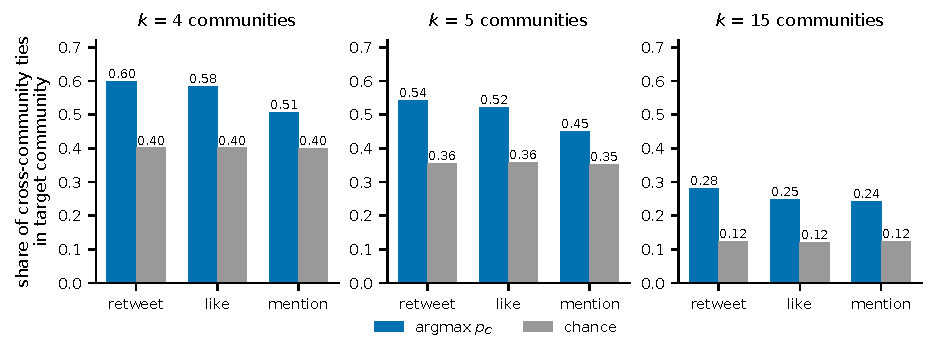
\includegraphics[width=\linewidth]{fig_e17.pdf}
\caption{Share of held-out cross-community ties of top-10\% misfits that land in the predicted community (bio-only text), by predictor, tie type and number of follow communities $k$. Graph-only predictors use the follow layer only.}
\label{fig:e17}
\end{figure}

\begin{table}[htbp]
\caption{Share of cross-community ties in the predicted community, TIMME, bio-only text. LP is one-step label propagation and AA is Adamic--Adar. The last column is text minus the strongest graph-only predictor in that row (named), with a 95\% paired bootstrap interval over users.}
\label{tab:e17}
\centering\small
\begin{tabularx}{\linewidth}{@{}cl cccccc >{\raggedright\arraybackslash}X@{}}
\toprule
$k$ & Tie & text & most-linked & LP & $p_T$ & AA & chance & text $-$ best graph-only [95\% CI]\\
\midrule
4 & retweet & 0.601 & 0.496 & 0.576 & 0.487 & 0.403 & 0.401 & LP: +0.025 [0.000, 0.053] \\
4 & like & 0.584 & 0.515 & 0.599 & 0.506 & 0.403 & 0.402 & LP: $-$0.015 [$-$0.042, 0.011] \\
4 & mention & 0.510 & 0.438 & 0.508 & 0.436 & 0.367 & 0.399 & LP: +0.002 [$-$0.020, 0.023] \\
\midrule
5 & retweet & 0.543 & 0.431 & 0.509 & 0.441 & 0.345 & 0.356 & LP: +0.034 [0.003, 0.064] \\
5 & like & 0.524 & 0.448 & 0.540 & 0.455 & 0.348 & 0.357 & LP: $-$0.016 [$-$0.044, 0.015] \\
5 & mention & 0.451 & 0.369 & 0.443 & 0.381 & 0.301 & 0.353 & LP: +0.008 [$-$0.016, 0.034] \\
\midrule
15 & retweet & 0.278 & 0.189 & 0.258 & 0.336 & 0.304 & 0.122 & $p_T$: $-$0.058 [$-$0.096, $-$0.019] \\
15 & like & 0.248 & 0.186 & 0.243 & 0.320 & 0.285 & 0.122 & $p_T$: $-$0.072 [$-$0.108, $-$0.036] \\
15 & mention & 0.242 & 0.165 & 0.216 & 0.267 & 0.245 & 0.123 & $p_T$: $-$0.025 [$-$0.051, 0.004] \\
\bottomrule
\end{tabularx}

\end{table}

\subsection{Rewiring toward the text-predicted community}
On the Pokec slice, Fig.~\ref{fig:e21} (right) and Table~\ref{tab:rew} show correction reach under the \meth{wc} model with $k{=}5$ rewires per misfit. At $\beta{=}6$, \meth{rehome\_text} raises reach from 50.34 to 61.26, a gain of +10.92 pp [9.76, 12.13] over no rewiring and +8.00 pp [6.87, 9.10] over \meth{random\_rewire}. Structural re-homing gives only +2.46 pp, no better than random rewiring (+2.92), and applying \meth{rehome\_text} to random nodes gives +0.63 [0.05, 1.31], so both the text target and the choice of misfits matter. The gain over random rewiring is clear from $\beta{=}1$ (+5.29 [3.98, 6.56]), and under the independent-cascade model (\meth{ic:2}) it is +8.68 [6.96, 10.65] at $\beta{=}6$. Total infected share is nearly unchanged (+0.110 pp). Caveat: $\beta$ is swept rather than measured.

\begin{figure}[htbp]
\centering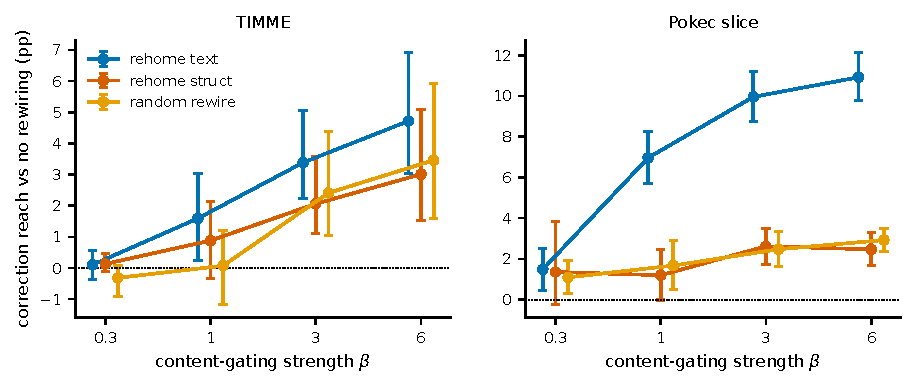
\includegraphics[width=\linewidth]{fig_e21.pdf}
\caption{Correction reach gain over no rewiring (pp, \meth{wc} model, $k{=}5$) versus content-gating $\beta$, with 95\% paired-bootstrap intervals over simulations (points offset horizontally for legibility). Left: TIMME (see Section~\ref{sec:niche}). Right: Pokec slice.}
\label{fig:e21}
\end{figure}

\begin{table}[htbp]
\caption{Correction reach at $\beta{=}6$ (\meth{wc}, $k{=}5$), reach in \% of nodes and contrasts in pp with 95\% bootstrap intervals.}
\label{tab:rew}
\centering\small
\begin{tabular}{@{}llccc@{}}
\toprule
Data & Method & Reach & vs none & vs random\_rewire\\
\midrule
TIMME & none & 34.54 & -- & -- \\
TIMME & rehome\_text (ours) & 39.25 & +4.72 [3.05, 6.91] & +1.26 [-0.33, 2.22] \\
TIMME & rehome\_struct & 37.55 & +3.01 [1.52, 5.08] & -0.45 [-1.84, 0.33] \\
TIMME & random\_rewire & 38.00 & +3.46 [1.59, 5.92] & -- \\
TIMME & rehome\_text, rand.\ nodes & 33.93 & -0.61 [-2.11, 0.17] & -4.07 [-6.90, -1.96] \\
\midrule
Pokec & none & 50.34 & -- & -- \\
Pokec & rehome\_text (ours) & 61.26 & +10.92 [9.76, 12.13] & +8.00 [6.87, 9.10] \\
Pokec & rehome\_struct & 52.81 & +2.46 [1.69, 3.29] & -0.46 [-1.27, 0.40] \\
Pokec & random\_rewire & 53.27 & +2.92 [2.36, 3.51] & -- \\
Pokec & rehome\_text, rand.\ nodes & 50.98 & +0.63 [0.05, 1.31] & -2.29 [-3.07, -1.44] \\
\bottomrule
\end{tabular}

\end{table}

\section{Further niche use cases}
\label{sec:niche}
The same score serves further tasks in specific scenarios. Table~\ref{tab:further} gives the winning number against its comparator and the scenario in which it holds; the paragraphs below say more.

\begin{table}[htbp]
\caption{Further use cases. Intervals 95\%.}
\label{tab:further}
\centering\small
\begin{tabular}{@{}>{\raggedright\arraybackslash}p{0.15\linewidth}>{\raggedright\arraybackslash}p{0.2\linewidth}>{\raggedright\arraybackslash}p{0.22\linewidth}>{\raggedright\arraybackslash}p{0.28\linewidth}@{}}
\toprule
Use & Ours & Comparator & Scenario where it works\\
\midrule
Party validation & AUC 0.682 & shuffled text 0.541; degree 0.361 & real party labels from bios\\
Blocking, misfit$\times$PR & +1.38 pts [0.40, 2.36] over best structural & best structural removes 33.0 pts & strong content gating ($\beta{=}6$), hub placement\\
Link friction & +14.9 pts [13, 16.8] over \meth{bridge\_struct} & \meth{bridge\_struct} & strong gating ($\beta{=}4$)\\
Planted detection & precision@20 0.787 [0.729, 0.846] & PageRank 0.0312 & planted mismatches, random or hub placement\\
Infiltrators & AUC 0.772 [0.752, 0.792] & betweenness 0.508 & text accuracy about 0.45 or higher\\
TIMME rewiring & +4.72 pp vs none [3.05, 6.91] & \meth{random\_rewire} +3.46 pp & strong content gating ($\beta{=}6$)\\
\bottomrule
\end{tabular}
\end{table}

\paragraph{Party validation (TIMME).}
On real TIMME accounts, misfit scores 0.682 AUC (one-sided $p{=}0.019$) for party-label mismatches, against 0.541 for a shuffled-text null and 0.361 for degree. It works when the party signal is present in the text; there are 11 positives among 595 labelled nodes.

\paragraph{Combining with centrality for blocking.}
Multiplying misfit by PageRank beats the best structural blocker by +1.38 pts [0.40, 2.36] in a synthetic cell with hub placement, $\beta{=}6$ and a 10\% mismatch share, where that blocker already removes 33.0 pts. It works when content gating is strong and the mismatched nodes are hubs.

\paragraph{Edge-level link friction.}
On synthetic graphs at $\beta{=}4$, \meth{bridge\_struct\_x\_recv} removes 14.9 pts [13, 16.8] more cross-community infection than \meth{bridge\_struct}. It works when receivers gate content strongly.

\paragraph{Detection on planted scenarios.}
Precision@20 on planted mismatches is 0.787 [0.729, 0.846] for misfit and 0.6375 for disagreement, against 0.0312 for PageRank; with hub placement it is 0.725 against 0.369 for PageRank. It works under both random and hub placement of the planted nodes.

\paragraph{Infiltrator detection.}
Misfit reaches 0.772 AUC [0.752, 0.792] against 0.508 for betweenness and 0.501 for PageRank and degree (text accuracy 0.61, random placement). It works for non-structural infiltrators when text accuracy is about 0.45 or higher.

\paragraph{Rewiring on TIMME.}
Rewiring misfits toward their text-predicted community gives +4.72 pp [3.05, 6.91] over no rewiring at $\beta{=}6$, against +3.46 pp for \meth{random\_rewire}; the text-specific margin over random rewiring is +1.26 [$-$0.33, 2.22]. It works when content gating is strong.
